\documentclass[11pt,a4paper]{article}
\usepackage[margin=2cm]{geometry}
\usepackage{float}
\usepackage{longtable}
\usepackage{tikz}
\usetikzlibrary{arrows.meta, positioning, shapes.geometric}
\usepackage{array}
\usepackage{amsmath}
\usepackage{ragged2e}
\usepackage{booktabs}
\usepackage{hyperref}
\usepackage{graphicx}
\graphicspath{{assets/}}
\usepackage{subcaption}
\usepackage{caption}
\usepackage{natbib}
\bibliographystyle{agsm}
\captionsetup[table]{font=footnotesize, labelfont=footnotesize, justification=centering}
\captionsetup[figure]{font=footnotesize, labelfont=footnotesize, justification=centering}
\newcolumntype{S}[1]{>{\scriptsize\raggedright\arraybackslash}p{#1}}
\newcolumntype{R}[1]{>{\RaggedRight\arraybackslash}p{#1}}
%-------------------------------------------------------------------------------
% Document information
%-------------------------------------------------------------------------------
% Use standard hyphen and new line separator.  The optional line break must
% be provided outside of math mode to avoid font warnings.
\title{Pipeline Documentation for Thesis \\[0.5em]
\large A structured description of the route-matching pipeline}
\author{\textbf{Author:} Jack Jibb}
\date{\today}

\begin{document}

\maketitle

\section*{Scope and purpose}
This document describes the end-to-end data processing pipeline contained in \texttt{pipeline}
directory.  The main purpose of the pipeline is to take a
GPS\footnote{GPS: Global Positioning System.} track stored in the GPS Exchange file
format (GPX), and produce a matched representation of that track on an
OpenStreetMap road network.  The result is an ordered sequence of matched
points and metadata that can be visualised and further analysed.  The
documentation follows established guidelines for software user documentation as
described in ISO/IEC/IEEE~26514\footnote{https://cdn.standards.iteh.ai/samples/77451/e161501288fd44f88c6fdd0f6e46b017/ISO-IEC-IEEE-26514-2022.pdf}.
The pipeline is a component of the larger route segmentation system and is designed to
be deployed as part of a web\,application backend. The code is already partly containerised
using Docker, and the exposed scripts will eventually become HTTP endpoints when integrated
into a web service. Recent development work has added native support for \emph{batch processing}:
instead of accepting only a single GPX file, the pipeline reads all files from a configurable
source directory and processes them concurrently.  This change means that multiple rides can be
matched to the map in one run, and each input file produces its own matched output and visualisation.
When ported to a web application, the same core code will be reused behind API endpoints that
interact with the different pipeline stages.

\section{Overview of the pipeline}
The pipeline is orchestrated by the Bash script \texttt{run\_pipeline.sh}, contained
in the \texttt{code/pipeline} directory. It reads settings from a YAML configuration file (\texttt{settings.yml})
and runs each component. The result of the pipeline is a matched GeoJSON route object that follows the path
that the GPX file is suggesting. This removes GPS error from noise, and provides a structured network that can be used in analysis.
Figures \ref{fig:gpx1} to \ref{fig:route2} show the comparison between mapped input GPX trackpoints and output GeoJSON route maps.
The pipeline stages are listed below; see
Figure~\ref{fig:flowchart} for a visual depiction.  Each step logs its
progress to the console, and the resulting artefacts are stored in the
\texttt{data/} sub-directory.

\begin{figure}[H]
	\centering

	% First row
	\begin{subfigure}[b]{0.48\textwidth}
		\centering
		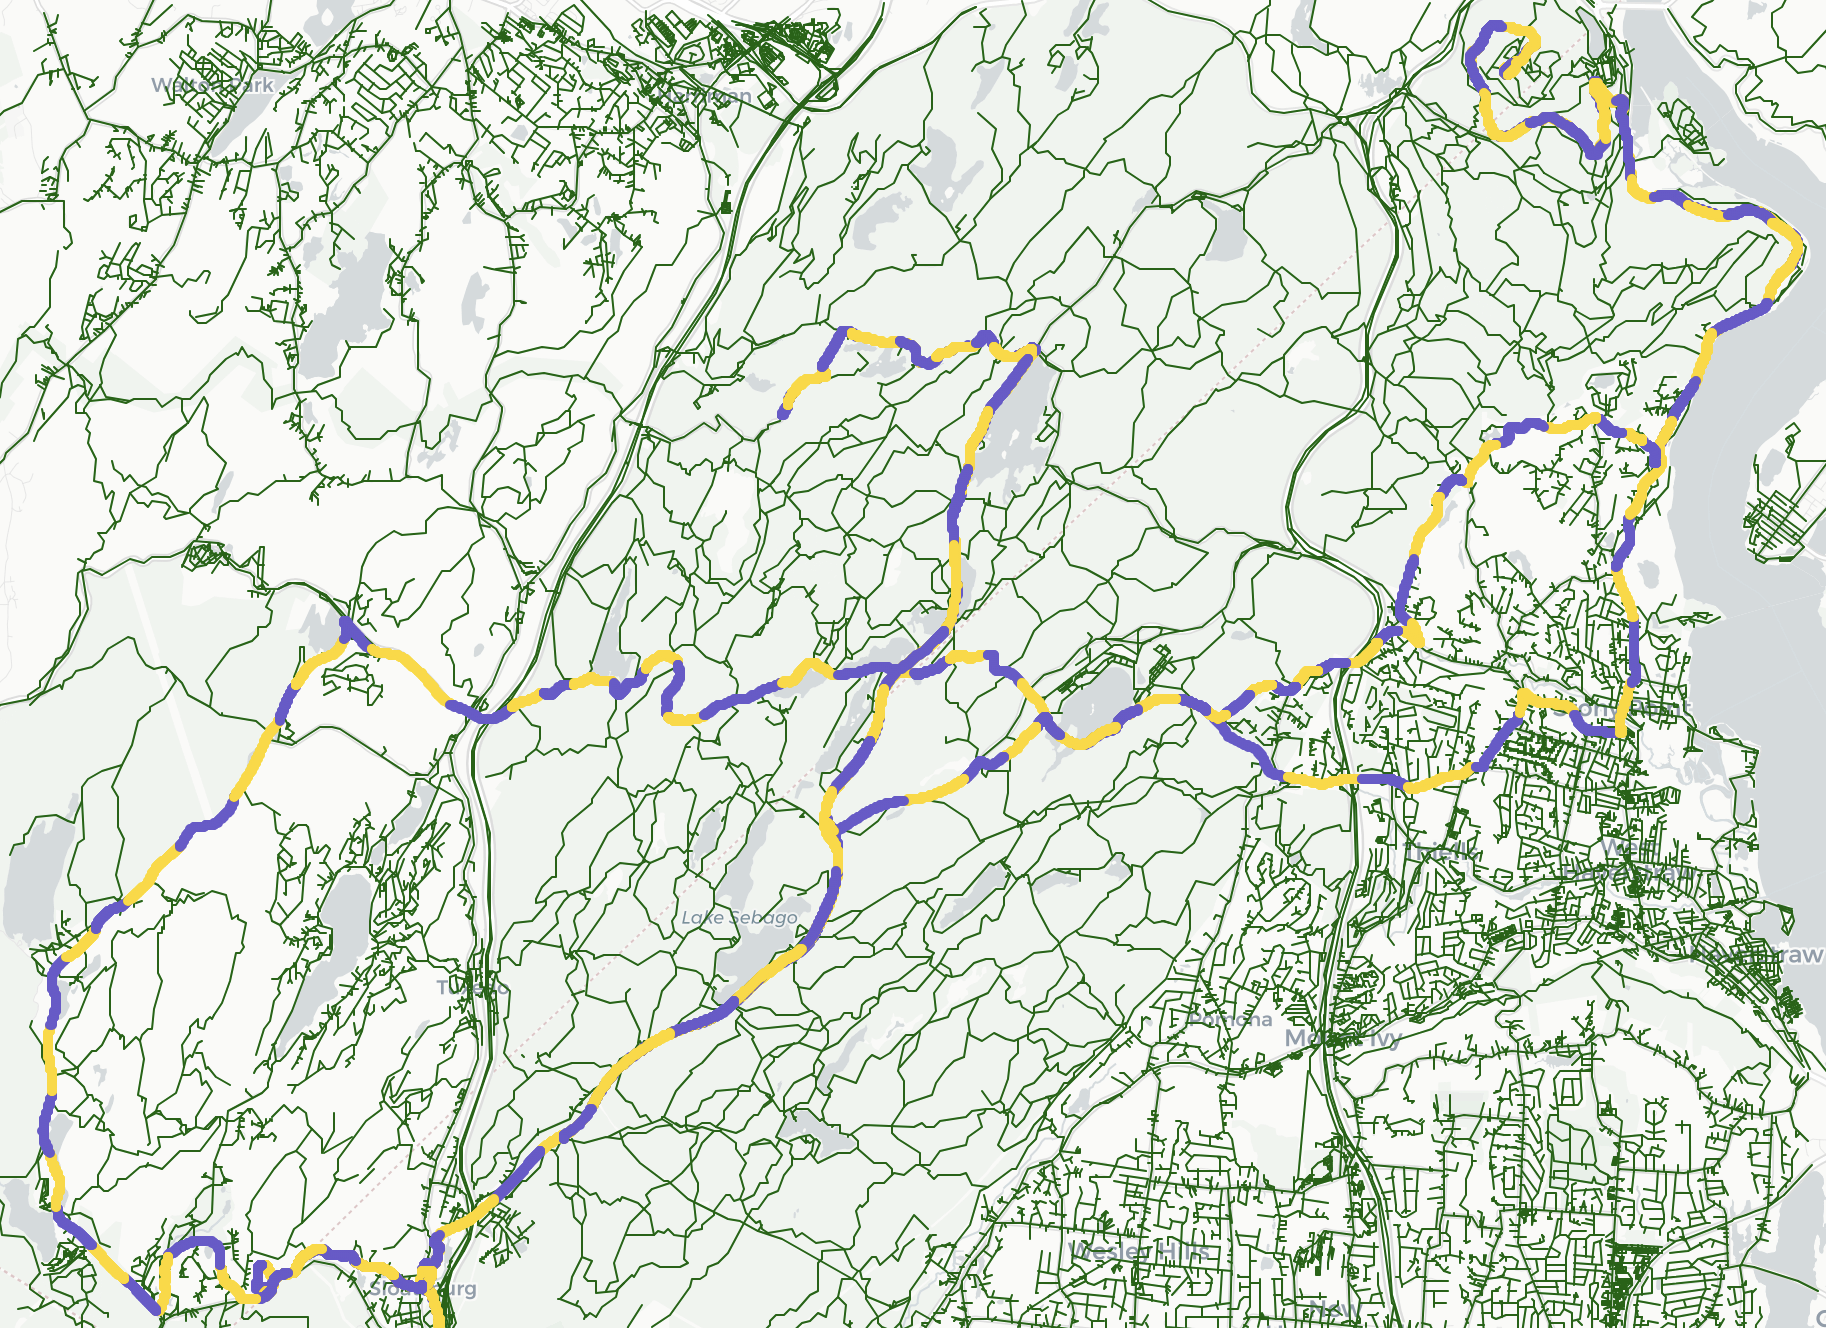
\includegraphics[width=\textwidth]{track1_gpx.png}
		\caption{Raw GPX track of whole file}
		\label{fig:gpx1}
	\end{subfigure}
	\hfill
	\begin{subfigure}[b]{0.48\textwidth}
		\centering
		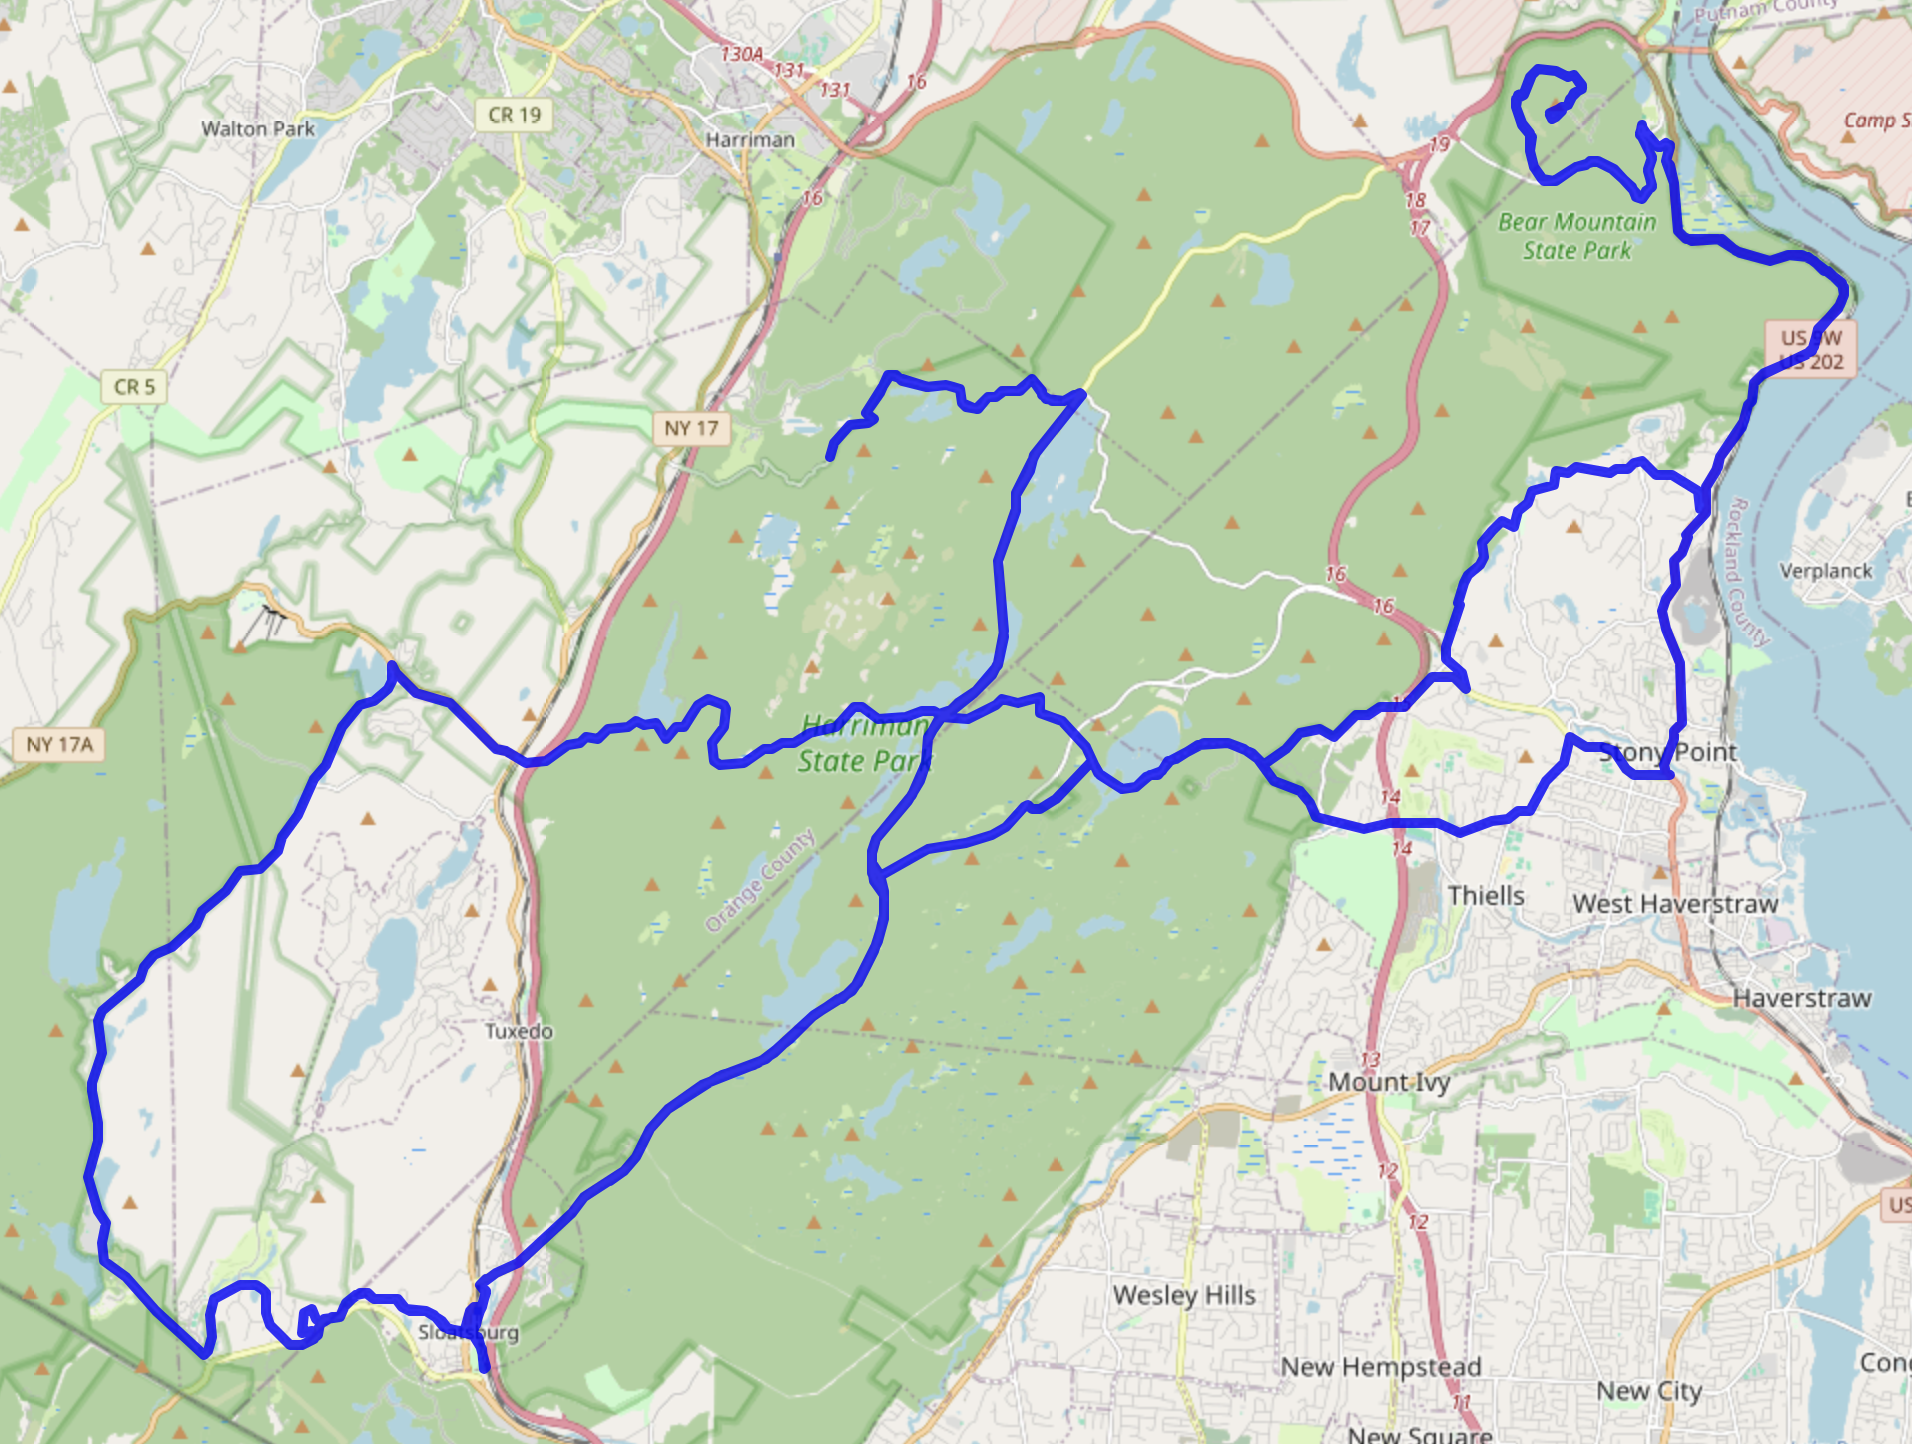
\includegraphics[width=\textwidth]{track1_route.png}
		\caption{Matched Route to whole file}
		\label{fig:route1}
	\end{subfigure}

	\par\bigskip % space between rows

	% Second row
	\begin{subfigure}[b]{0.48\textwidth}
		\centering
		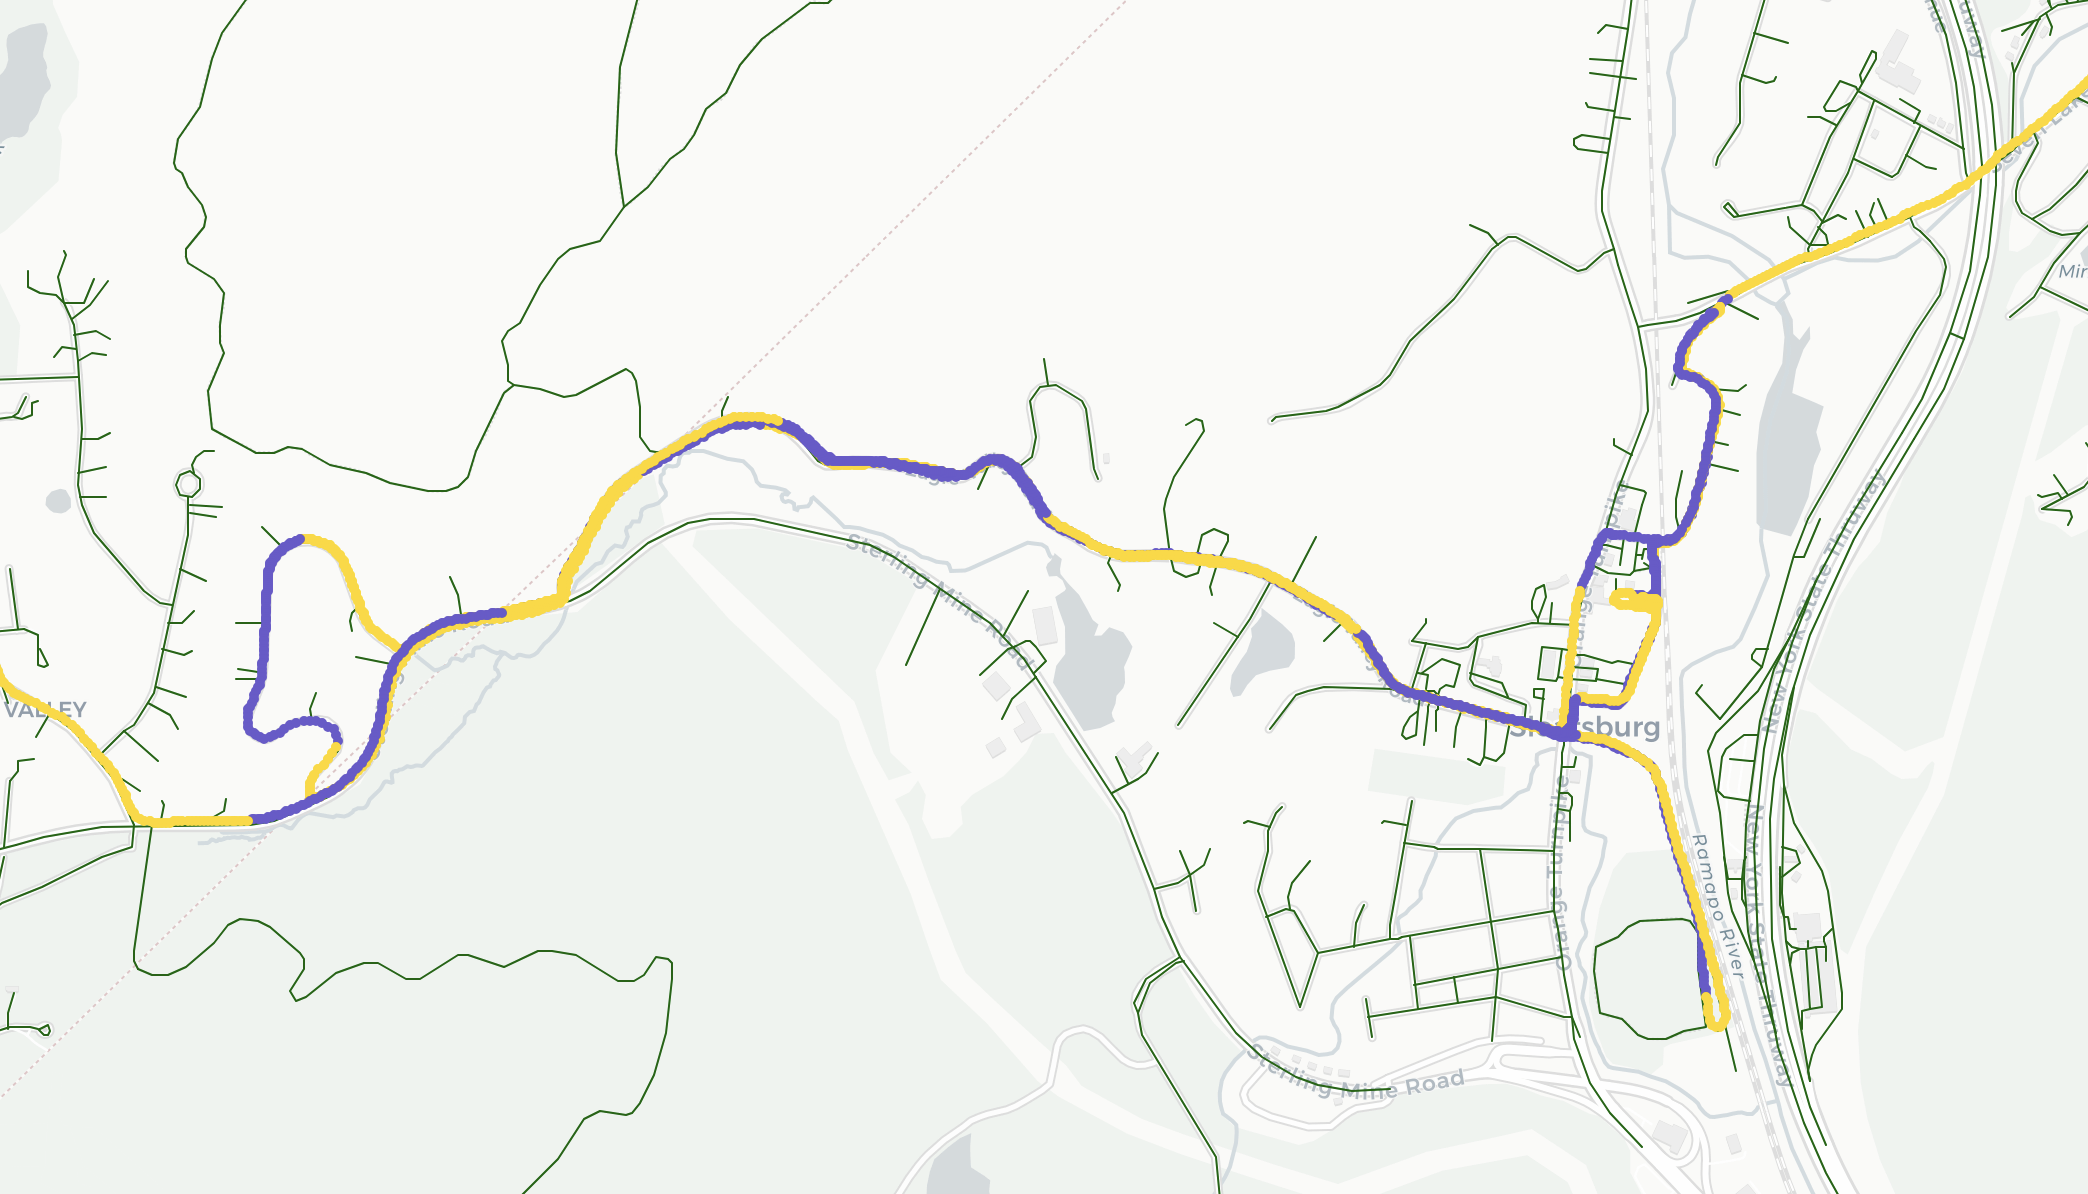
\includegraphics[width=\textwidth]{track2_gpx.png}
		\caption{A detailed subsection of GPX trackpoints}
		\label{fig:gpx2}
	\end{subfigure}
	\hfill
	\begin{subfigure}[b]{0.48\textwidth}
		\centering
		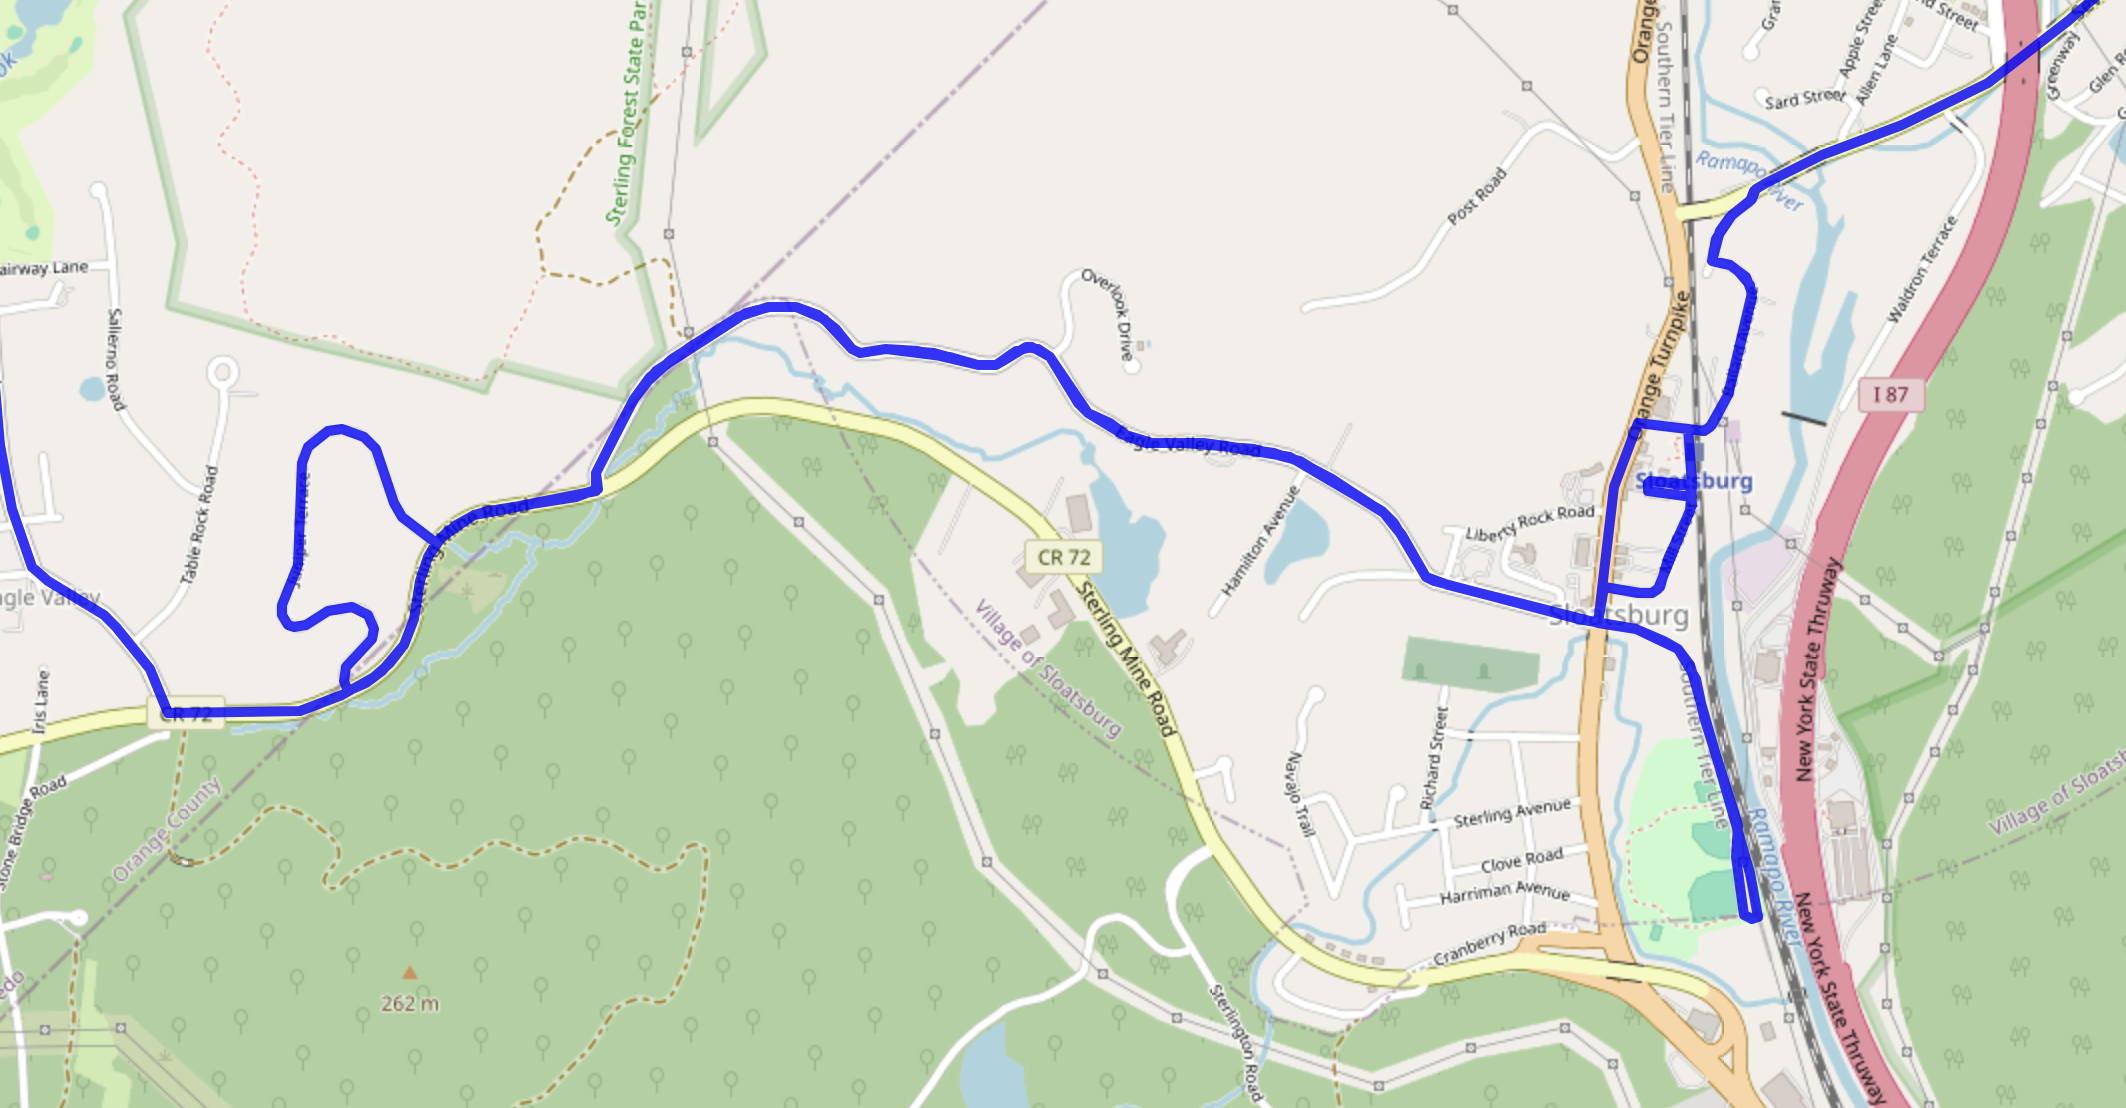
\includegraphics[width=\textwidth]{track2_route.png}
		\caption{The same area, in GeoJSON route form}
		\label{fig:route2}
	\end{subfigure}

	\caption{Comparison of raw GPX tracks and OSRM-matched routes: (a) GPX Track 1, (b) Route 1, (c) GPX Track 2, (d) Route 2.}
	\label{fig:gpx_vs_route_grid}
\end{figure}

\subsection{Description of pipeline processing steps}
\begin{enumerate}
	\item \textbf{Configuration loading}---The script reads \texttt{settings.yml} to load initial settings for the pipeline.
	      This includes (\texttt{gpx\_source}) where the pipeline looks for .gpx files, and (\texttt{/osm\_files}) the directory where downloaded OpenStreetMap \texttt{.osm} files are stored.
	      It also loads some other options, such as the size of the "chunks" (defined later) that the program splits each GPX file into.
	\item \textbf{Environment setup}---A Python virtual environment is created (if
	      it does not already exist) and dependencies from
	      \texttt{requirements.txt} are installed.  This isolates the pipeline from
	      the system environment, and any future upgrades or dependency updates can be
	      managed through this step.
	\item \textbf{Data extraction and map download}---The shell script\footnote{The call is performed using Python's \texttt{subprocess}
		      module within \texttt{run\_pipeline.sh}; for brevity the exact command is not reproduced here.
		      See Appendix (Code Section) for the full shell script} invokes the Python module \texttt{prepare\_map.py}.
	      In the current version the input to this module is a \emph{directory} of GPX files.  The script enumerates all
	      \texttt{.gpx} files in the directory and, using a thread pool, performs the following steps for each file:
	      \begin{itemize}
		      \item Parses the GPX track to obtain a sequence of latitude/longitude/timestamp points
		      \item Computes a bounding box around the full gps track and downloads the OpenStreetMap .osm file for the bbox from the Overpass API \cite{overpass},
		            saving it as \texttt{\textless gpx\_name\textgreater{}.osm} in the directory defined by \texttt{osm\_files}.
		      \item Converts the track points into one or more OSRM GeoJSON objects and writes them to \texttt{data/temp/\textless gpx\_name\textgreater{}}.
		            Each JSON file represents a ``chunk''\footnote{Chunking is necessary to avoid exceeding URL length limits when later calling the OSRM \texttt{/match} API, which accepts only HTTP GET requests.}
		            of at most \texttt{chunk\_size} points (a value of~0 in \texttt{settings.yml} disables chunking).
	      \end{itemize}
	\item \textbf{Conversion of OpenStreetMap data to Protocolbuffer Binary Format (.pbf)}---\\Within a Docker container, the \texttt{osmium}
	      tool converts the \texttt{.osm} files into the more compact \texttt{.pbf} format.
	      When multiple extracts have been downloaded (one per GPX file), they are merged into a single \texttt{merged.pbf} via the scripts
	      located in \texttt{osmium/scripts}.
	      The resulting file is renamed \texttt{map.pbf} and stored in \texttt{data/osrm\_map/}, and the indidual \texttt{.pbf} fragments are removed.
	\item \textbf{Graph preparation with Docker}---Docker Compose is used to containerize the OSRM\footnote{OSRM: Open Source Routing Machine.} backend.
	      The \texttt{osrm-prep} service preprocesses the \texttt{map.pbf} using the custom cycling profile in \texttt{docker/osrm/profile.lua}
	      to build the routing graph.  Once preprocessing completes, the \texttt{osrm-server} service is launched in detached mode,
	      exposing the \texttt{/match} endpoint on port~5000, ready for route matching.
	\item \textbf{Route matching}---For each GPX file, the script invokes \texttt{batch\_route\_calc.py} on its
	      corresponding chunk directory.  This module reads the OSRM JSON chunks in their directories and performs parallel requests to the OSRM
	      \texttt{/match} API using a thread pool.  Each request uses a \emph{dynamic radius algorithm} that increases the search radius per track point
	      when the heading (direction) of the track has a high variance. This gives more context for \texttt{/match's} algorithm to decide whether to turn off a road or not.
	      The results of successful matches are saved as \texttt{result\_*.json} files in \texttt{data/results/\textless gpx\_name\textgreater{}},
	      while failures are saved to a \texttt{gap/} subdirectory for later gap filling using the \texttt{/route}\footnote{The \texttt{/route}
		      endpoint calculates the path between two coordinates based on criteria such as distance or duration} endpoint.
	\item \textbf{Merging}---Once all chunks for a GPX file have been processed, \texttt{merge\_routes.py} recursively combines
	      individual matching results into a single route.  The merge logic decodes the geometries, concatenates all data arrays in the file,
	      and computes aggregate distance and duration values.  Merging is multi‑threaded per recursion instance, and produces a single JSON file named after
	      the input GPX file (e.g., \texttt{\textless gpx\_name\textgreater{}.json}) saved directly in \texttt{data/results}.  After merging,
	      the per‑file result chunks and their directories are removed.
	\item \textbf{Visualisation}---Finally, \texttt{plot\_merged.py} iterates over the merged JSON files in
	      \texttt{data/results}, creating a Folium map for each route. The purpose of the map is mostly used for debugging the code, as the main goal
	      of the pipeline is to generate a continuous route that matches the GPX route as closely as possible. Each map can optionally
	      overlay the raw GPS points for accuracy checking.  The outputs are saved as
	      \texttt{\small interactive\_map\_\textless gpx\_name\textgreater{}.html} per input file,
	      which can be opened in a web browser to inspect the matched route. This html can be served once the program is
	      implemented into a web back-end, as a debug option.
	\item \textbf{Clean\,up}---Temporary files (the intermediate JSON chunks, fragment \texttt{.pbf} files for individual gpx files and
	      Docker volumes) are deleted.  The virtual environment is deactivated and the OSRM containers are stopped and removed using Docker Compose.
	      The script leaves the virtual environment directory intact so that subsequent runs reuse the existing dependencies.
\end{enumerate}
\begin{figure}[H]
	\centering
	\scalebox{0.85}{
		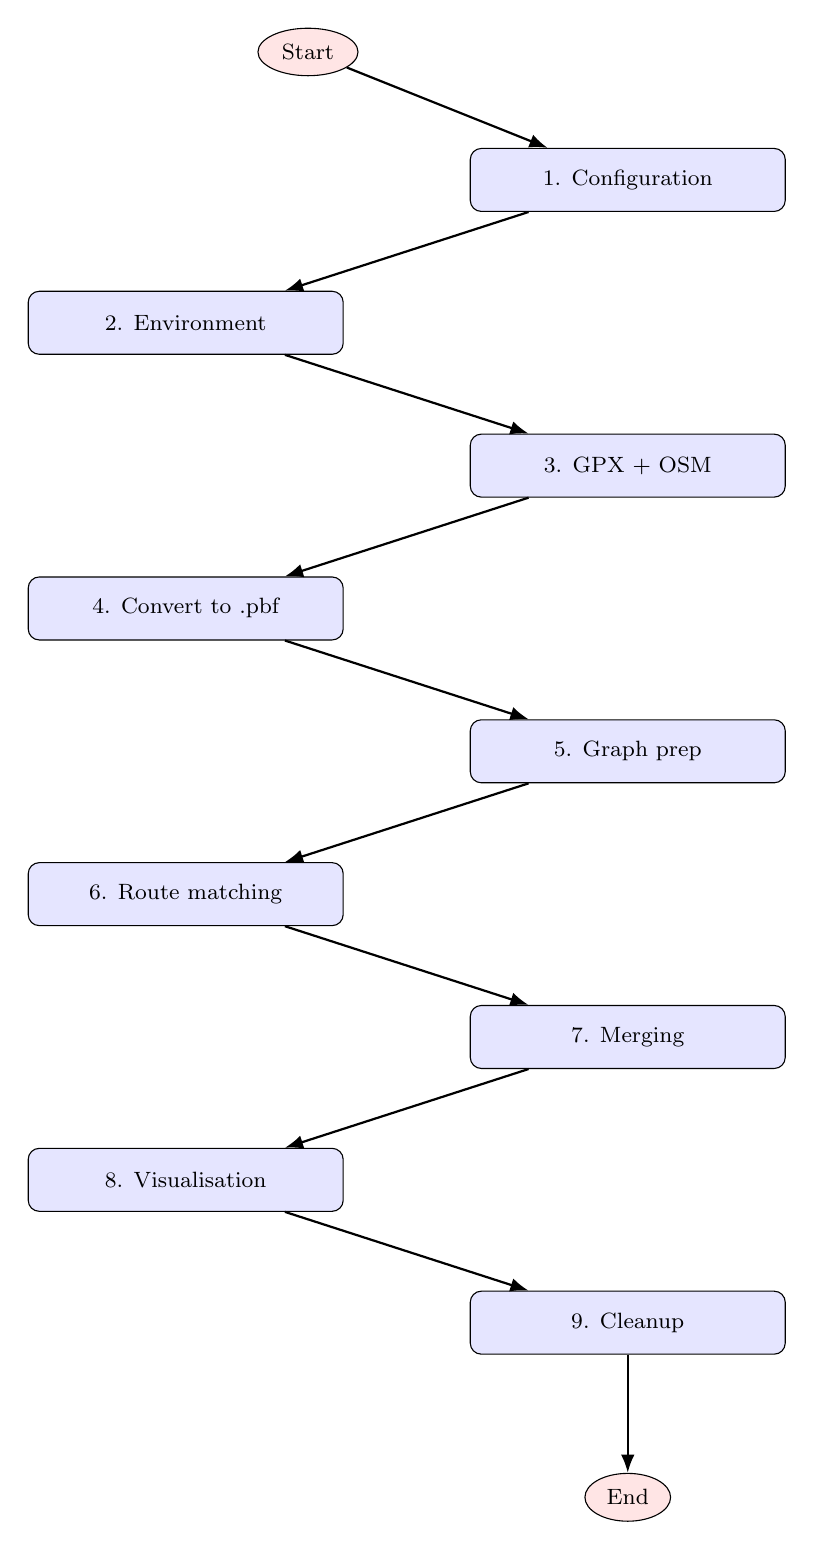
\begin{tikzpicture}[
			node distance=1.0cm and 1.6cm,
			every node/.style={font=\footnotesize},
			process/.style={rectangle, draw, rounded corners, align=center, minimum width=4.0cm, minimum height=.8cm, fill=blue!10},
			startstop/.style={ellipse, draw, align=center, fill=red!10},
			arrow/.style={-{Latex}, thick}
			]

			\node[startstop] (start) {Start};
			\node[process, below right=of start] (config) {1. Configuration};
			\node[process, below left=of config] (env) {2. Environment};
			\node[process, below right=of env] (extract) {3. GPX + OSM};
			\node[process, below left=of extract] (convert) {4. Convert to .pbf};
			\node[process, below right=of convert] (graph) {5. Graph prep};
			\node[process, below left=of graph] (match) {6. Route matching};
			\node[process, below right=of match] (merge) {7. Merging};
			\node[process, below left=of merge] (viz) {8. Visualisation};
			\node[process, below right=of viz] (cleanup) {9. Cleanup};
			\node[startstop, below=1.5cm of cleanup] (end) {End};

			\draw[arrow] (start) -- (config);
			\draw[arrow] (config) -- (env);
			\draw[arrow] (env) -- (extract);
			\draw[arrow] (extract) -- (convert);
			\draw[arrow] (convert) -- (graph);
			\draw[arrow] (graph) -- (match);
			\draw[arrow] (match) -- (merge);
			\draw[arrow] (merge) -- (viz);
			\draw[arrow] (viz) -- (cleanup);
			\draw[arrow] (cleanup) -- (end);

		\end{tikzpicture}
	} % CLOSE the scalebox here!
	\caption{Pipeline flowchart for the GPX to OSRM-matched route processing system.}
	\label{fig:flowchart}
\end{figure}
\section{Component Overview}
The pipeline comprises several scripts and modules.  Table~\ref{tab:modules}
summarises their roles and highlights their main functions.

\begin{longtable}{
	@{}
	>{\scriptsize\raggedright\arraybackslash}p{3cm}   % tiny + ragged-right
	p{8cm}                                             % normal justified
	>{\scriptsize\RaggedRight\arraybackslash}p{4cm}               % normal + ragged-right
	@{}
	}
	\caption{\footnotesize Summary of key modules in the pipeline.  The descriptions focus on
		the primary purpose of each module and list notable functions exposed for
	reuse.\label{tab:modules}}                                                                                                                                                  \\
	\toprule
	\textbf{Module/file}                                                     & \textbf{Purpose}                                            & \textbf{Notable functions/scripts} \\
	\midrule
	\endfirsthead
	\multicolumn{3}{c}%
	{{\bfseries Table~\thetable\ continued from previous page}}                                                                                                                 \\
	\toprule
	\textbf{Module/file}                                                     & \textbf{Purpose}                                            & \textbf{Notable functions/scripts} \\
	\midrule
	\endhead
	\midrule \multicolumn{3}{r}{\emph{Continued on next page}}                                                                                                                  \\
	\endfoot
	\bottomrule
	\endlastfoot	\texttt{run\_pipeline.sh}                                   & Orchestrates the entire pipeline, loading
	configuration values from \texttt{settings.yml}, creating a virtual
	environment, invoking the Python scripts, running Docker containers for
	\texttt{osmium} and OSRM, and performing clean-up.                       & Shell script; calls
	\texttt{python3 source/prepare\_map.py}, \texttt{python3
		source/batch\_route\_calc.py}, \texttt{python3 source/merge\_routes.py} and
	\texttt{python3 source/plot\_merged.py}.                                                                                                                                    \\
	\texttt{prepare\_map.py}                                                 & Parses all GPX files in a directory, extracts track points,
	calculates a bounding box and downloads the corresponding OpenStreetMap extract
	from the Overpass API.  Converts the track points into GeoJSON files,
	supporting optional chunking.                                            & \texttt{parse\_args()},
	\texttt{main()}; uses \texttt{utils.gpx\_utils} and
	\texttt{utils.osrm\_utils}.                                                                                                                                                 \\
	\texttt{batch\_route\_calc.py}                                           & Reads the OSRM JSON chunks and performs
	concurrent map matching requests to a containerized OSRM server. Uses polyline to compress coordinate data, and writes the matching results to
	\texttt{result\_*.json}.                                                 &
	\texttt{get\_osrm\_match()}, \texttt{format\_list()}, \texttt{main()}                                                                                                       \\
	\texttt{merge\_routes.py}                                                & Merges multiple matched segments into a single
	route using a recursive "tree merge" algorithm.  Combines distances,
	durations and geometries while maintaining order.                        &
	\texttt{merge\_two()}, \texttt{tree\_merge\_routes()}, \texttt{main()}                                                                                                      \\
	\texttt{plot\_merged.py}                                                 & Generates an interactive map (HTML) of the
	merged route using Folium.  Alternates colours for different segments and
	optionally overlays raw points for comparison.                           & \texttt{main()}; uses
	\texttt{folium}, \texttt{itertools.cycle}                                                                                                                                   \\
	\texttt{utils/gpx\_utils.py}                                             & Provides helper functions for reading GPX files,
	computing bounding boxes, downloading OSM extracts and serialising data to
	JSON.                                                                    & \texttt{load\_gpx()}, \texttt{bounding\_box\_from\_data()},
	\texttt{download\_osm\_file()}, \texttt{extract\_data\_from\_gpx()}                                                                                                         \\
	\texttt{utils/osrm\_utils.py}                                            & Defines functions to convert GPX points into
	OSRM JSON payloads, calculate adaptive radii based on heading changes and
	remove spurious segments.  Also includes helpers for reading OSM bounds. &
	\texttt{points\_to\_osrm\_json()}, \texttt{compute\_dynamic\_radius()},
	\texttt{prune\_spurs()}                                                                                                                                                     \\
	\texttt{docker/docker-compose.yml}                                       & Describes the Docker services used for
	conversion and map matching.  Defines an \texttt{osmium} service for
	converting \texttt{.osm} files to \texttt{.pbf}, an \texttt{osrm-prep}
	service for building the routing graph and an \texttt{osrm-server} service
	that exposes the \texttt{/match} endpoint on port~5000.                  & YAML file; run
	with \texttt{docker compose}                                                                                                                                                \\
	\bottomrule
\end{longtable}
\section{Python Module Breakdown}

\subsection{GPX Utilities (\texttt{gpx\_utils.py})}

This module provides low-level helpers for GPX parsing, bounding-box computation, JSON I/O, and OSM downloads.

\paragraph{load\_gpx(path)}
Opens and parses a GPX file using \texttt{gpxpy.parse()}, returning a \texttt{GPX} object with tracks, segments, and points.
\emph{Citation:} \citep{gpxpy}

\paragraph{extract\_data\_from\_gpx(gpx)}
Iterates through \texttt{gpx.tracks} → \texttt{.segments} → \texttt{.points}, building a list of dictionaries with:
\begin{itemize}
	\item \texttt{lat}, \texttt{lon}: coordinates
	\item \texttt{elv}: elevation (or \texttt{None})
	\item \texttt{time}: ISO-formatted timestamp
	\item any GPX \texttt{pt.extensions}, flattened into key–value pairs. Including but not limited to: Power, Cadence, Heartrate, and Temperature.
\end{itemize}
This list will be the heart of the categorization section of the program, as it contains all rider-specific metadata.

\paragraph{bounding\_box\_from\_data(data)}
Given a list of point dicts, extracts all latitudes and longitudes, computes:
\[
	\text{south} = \min(\mathrm{lats}), \quad
	\text{north} = \max(\mathrm{lats}),\quad
	\text{west}  = \min(\mathrm{lons}),\quad
	\text{east}  = \max(\mathrm{lons}),
\]
and returns the bbox tuple \((\text{south},\text{west},\text{north},\text{east})\).

\paragraph{bbox\_contains(outer, inner)}
Checks that the inner bbox lies fully within the outer by comparing numeric bounds:
\begin{align*}
	\min(\mathrm{lat}_{\mathrm{inner}}) & \ge \min(\mathrm{lat}_{\mathrm{outer}})\;\wedge{} \\
	\min(\mathrm{lon}_{\mathrm{inner}}) & \ge \min(\mathrm{lon}_{\mathrm{outer}})\;\wedge{} \\
	\max(\mathrm{lat}_{\mathrm{inner}}) & \le \max(\mathrm{lat}_{\mathrm{outer}})\;\wedge{} \\
	\max(\mathrm{lon}_{\mathrm{inner}}) & \le \max(\mathrm{lon}_{\mathrm{outer}})
\end{align*}

Returns \texttt{True}/\texttt{False}.


\paragraph{load\_json(file\_path)}
Reads and parses a JSON file via \texttt{json.load()}.
\emph{Citation:} \citep{python-json-doc}

\paragraph{write\_json(points, path)}
Ensures the target directory exists (\texttt{os.makedirs(..., exist\_ok=True)}), then writes \texttt{points} with \texttt{json.dump(separators=(",", ":"), ensure\_ascii=False)} for compact output.

\paragraph{download\_osm\_file(bbox, output\_path)}
Constructs an Overpass “map” query URL of the form
\texttt{https://overpass-api.de/api/map?bbox=west,south,east,north},
fetches via \texttt{requests.get()}, and writes the raw OSM XML to disk.
\emph{Citations:} \citep{overpass-api-doc,python-requests-doc}

\vspace{1ex}\noindent
This module will also be used in the segmentation algorithm, but the relevant functions will be described in the Segmentation Algorithm documentation

\subsection{Data Extraction and Map Download (\texttt{prepare\_map.py})}

The \texttt{prepare\_map.py} module handles reading raw GPX tracks and fetching the corresponding OpenStreetMap extracts.  It defines four primary functions:

\paragraph{parse\_args()}
Uses Python’s \texttt{argparse} library to define and parse the command‐line interface \citep{python-argparse-doc}.
\begin{itemize}
	\item \texttt{gpx\_file\_path}: Input directory containing one or more \texttt{.gpx} files.
	\item \texttt{osm\_output\_path}: Directory in which to save downloaded \texttt{.osm} files.
	\item \texttt{radius}: Search radius (in metres) used for each track point.
	\item \texttt{chunk\_size}: Maximum number of GPS points per OSRM JSON chunk (0 = no chunking).
\end{itemize}

\paragraph{thread\_processes(gpx\_file, output\_path, chunk\_dir, radius, chunk\_size)}
Executed concurrently for each GPX file via \texttt{ThreadPoolExecutor} \citep{python-concurrent-doc}:
\begin{enumerate}
	\item \textbf{Load and parse GPX:}
	      Calls \texttt{load\_gpx(gpx\_file)} and \texttt{extract\_data\_from\_gpx(gpx)} from the \texttt{gpxpy} library to obtain a list of \{lat, lon, timestamp\} tuples \citep{gpxpy}.
	\item \textbf{Prepare output paths:}
	      Derives \texttt{gpx\_name} via \texttt{os.path.splitext} and ensures \texttt{output\_path} exists using Python’s \texttt{os} module \citep{python-os-doc}.
	\item \textbf{Chunk for OSRM:}
	      Invokes \texttt{points\_to\_osrm\_json(points, chunk\_dir, gpx\_name, radius, chunk\_size)} (in \texttt{utils/osrm\_utils.py}) to split the track into one or more JSON payloads ready for OSRM’s \texttt{/match} endpoint.
	\item \textbf{Fetch OSM if needed:}
	      If \texttt{\textless gpx\_name\textgreater{}.osm} does not already exist under \texttt{output\_path}, calls \texttt{get\_single\_osm\_from\_gpx()}, otherwise logs a warning and skips.
\end{enumerate}

\paragraph{get\_single\_osm\_from\_gpx(gpx\_file, points, gpx\_name, output\_path)}
Retrieves OSM data via the Overpass API \citep{overpass-api-doc}:
\begin{itemize}
	\item \textbf{Compute bounding box:}
	      Uses \texttt{bounding\_box\_from\_data(points)} (from \texttt{utils/gpx\_utils.py}) to derive the min/max latitude and longitude.
	\item \textbf{(Re)load GPX points:}
	      Calls \texttt{load\_gpx()} and \texttt{extract\_data\_from\_gpx()} again to ensure consistency.
	\item \textbf{Download OSM file:}
	      Invokes \texttt{download\_osm\_file(bbox, full\_output\_path)}, which constructs an Overpass API query and writes the resulting \texttt{.osm} XML to disk.
\end{itemize}

\paragraph{main()}
Orchestrates the module workflow:
\begin{itemize}
	\item Parses CLI arguments via \texttt{parse\_args()}.
	\item Scans \texttt{gpx\_file\_path} for \texttt{.gpx} files using \texttt{os.listdir()} and \texttt{os.path.isfile()} \citep{python-os-doc}.
	\item Determines \texttt{MAX\_THREADS} as \(\min(32, \text{number of GPX files})\).
	\item Creates a \texttt{ThreadPoolExecutor(max\_workers=MAX\_THREADS)} and submits \texttt{thread\_processes()} tasks for each GPX file.
	\item Uses \texttt{as\_completed()} to wait for all threads to finish before exiting.
\end{itemize}

\vspace{1ex}\noindent
This design parallelizes I/O and network operations, which are the most time-costly operations.




\section{Configuration options}
The pipeline reads configuration values from \texttt{settings.yml}.  Table~\ref{tab:settings}
summarises the available keys and their meanings.  Ensure that file paths
refer to existing locations and that chunk sizes remain within reasonable
limits to avoid exceeding URL length limits when calling the OSRM API.

\begin{longtable}{@{}>{\footnotesize\ttfamily}p{4cm}p{9cm}@{}}	\caption{Summary of configuration keys in \texttt{settings.yml}.\label{tab:settings}}                                                                                       \\
	\toprule
	\textbf{Key}                     & \textbf{Description}                                                                                                                                                                   \\
	\midrule
	\endfirsthead
	\multicolumn{2}{c}%
	{{\bfseries Table~\thetable\ continued from previous page}}                                                                                                                                                               \\
	\toprule
	\textbf{Key}                     & \textbf{Description}                                                                                                                                                                   \\
	\midrule
	\endhead
	\midrule \multicolumn{2}{r}{\emph{Continued on next page}}                                                                                                                                                                \\
	\endfoot
	\bottomrule
	\endlastfoot
	\texttt{gpx\_source}             & Directory containing one or more GPX files.  All files with the \texttt{.gpx} extension in this directory will be processed.  Example: \texttt{data/input}.                            \\
	\texttt{chunk\_size}             & Maximum number of points per OSRM JSON file.  A value of 0 disables chunking.  Large values may exceed the URL length limit of the OSRM API; the script enforces a maximum of 200.     \\
	\texttt{radius}                  & Initial search radius (in metres) used when matching points to the road network.  The dynamic radius algorithm may adjust this value on a per‑point basis.  Example: \texttt{5}.       \\
	\texttt{dynamic\_radius\_window} & Size of the initial sliding window used when computing dynamic radii.  Larger values smooth the radius changes over more points; smaller values react more quickly to heading changes. \\
\end{longtable}

\section{Running the pipeline}
This section provides a step-by-step procedure for executing the pipeline.  It
assumes that both Docker and Python 3.10 or higher are installed on the host
system.

\begin{enumerate}
	\item \textbf{Clone the repository} if you have not already done so.  In
	      a terminal, run:\\
	      % escape ampersands for LaTeX alignment
	      \texttt{\small git clone https://github.com/jibb34/MScProject \&\& cd MScProject/code/pipeline}\\
	      This will put you into the main pipeline directory, and you can see all the files and subdirectories with: \texttt{ls -la .}
	\item \textbf{Inspect and modify \texttt{settings.yml}} to set \texttt{gpx\_source} to the directory containing your GPX files and adjust parameters as needed.  Do not exceed a chunk size of
	      200 points.  If necessary, increase the search radius if the file contains a lot of GPS noise
	\item \textbf{Execute the pipeline} by running the shell script:
	      \begin{quote}
		      \texttt{bash ./run\_pipeline.sh}
	      \end{quote}
	      The script will create a Python virtual environment, install
	      dependencies, download the map, build the OSRM graph and perform route
	      matching.  Progress messages are printed to the console. While the script is running,
	      do not attempt to modify any files or paths in the main \texttt{pipeline} directory
	\item \textbf{View the results}.  After the script completes, open all
	      \texttt{\small interactive\_map\_\textless gpx\_name\textgreater{}.html} files (one file per input GPX) in a web browser.  The file is
	      located in the main directory.  You can also inspect
	      the merged JSON files for a structured representation of the matched
	      route. They are located in \texttt{./data/results}
	\item \textbf{Clean up}.  The script performs clean-up automatically.
	      Temporary files are removed and containers are shut down. If you wish to start a clean
	      run, you may delete the \texttt{.venv} directory to remove the python environment, and
	      you should delete all html files and GeoJSON files with this command:\\
	      \texttt{rm -rf .venv ./data/results/* ./*.html}
\end{enumerate}

\section{Error handling and warnings}
The pipeline contains the following safeguards:
\begin{itemize}
	\item If \texttt{settings.yml} is missing or lacks required keys, the script
	      exits immediately with an error message.
	\item The chunk size is validated to ensure it does not exceed 200 points.
	      Exceeding this limit may produce URLs that are too long for the OSRM
	      server to process; a fatal error is raised if the limit is broken.
	\item Requests to the OSRM server are wrapped in exception handling.  If a
	      request fails (e.g., network error), an empty result is produced and
	      saved to a \texttt{gap/} directory for later gap filling. This will be implemented
	      later for more robust behaviour if necessary. I have not had any empty requests
	      that were not a part of programmatic errors.
	\item During merging, the script checks for missing geometries or mismatched
	      code values and reports errors if encountered.  Merging proceeds even
	      when some segments cannot be combined, but is flagged as incomplete.
	\item If the Folium plotting script cannot find any match result files, it
	      raises an explicit \texttt{FileNotFoundError}.
\end{itemize}

% \section{Suggested figures and photographs}
% Figures enhance understanding of the pipeline.  The following photographs or
% screenshots can be inserted once you run the program.  Save each image as a
% \texttt{.png} file in the \texttt{figures/} directory and reference it using
% \verb|\includegraphics| in your LaTeX document.
% \begin{itemize}
% 	\item \textbf{Dynamic radius plot}---If you instrument the code to record
% 	      dynamic radii, plot a simple chart showing how the radius varies along
% 	      a track segment.  This helps readers understand the purpose of the
% 	      adaptive radius algorithm.
% \end{itemize}

\section*{References}
\begin{thebibliography}{9}
	\bibitem{overpass} Overpass API, \emph{OpenStreetMap data extractor},
	\url{https://overpass-api.de} (accessed August~2025).
	\bibitem{iso26514} ISO/IEC/IEEE~26514:2008, \emph{Systems and software
		engineering--Requirements for designers and developers of user documentation}.
\end{thebibliography}

\end{document}


